\documentclass[a4paper]{article}
\usepackage{times}
\usepackage[utf8]{inputenc}
\usepackage[T1]{fontenc}
\usepackage{graphicx}
\usepackage{amssymb}
\usepackage{hyperref}
\linespread{1.5}	% double spaces lines
\usepackage[hmargin=3cm,vmargin=3cm]{geometry}
\usepackage{indentfirst}
\usepackage{amsmath}
\usepackage{amsthm}
\usepackage{sectsty}
\usepackage{enumitem}
\usepackage[brazil]{babel}
\usepackage{placeins} %mantem figuras na secao com \FloatBarrier
\usepackage{fixltx2e} %\textsubscript
\usepackage{textcomp}
\hypersetup{%
    pdfborder = {0 0 0}
}

\begin{document}

\begin{titlepage}
\begin{center}


\large{ 
\uppercase{ Universidade Federal do Rio Grande do Sul\\

Instituto de Informática \\

Curso de Ciência da Computação \\

Circuitos Digitais (2014/1)\\
}

Prof. Dr. Marcelo de Oliveira Johann \\

Graduandos: \\ Paulo Renato Lanzarin (228818)
			\\ Ricardo Gabriel Herdt (160622) \\ [4.5cm]


% Title
\LARGE {\bfseries Relatório do laboratório 06: \\
	Projeto de um decodificador para 7 segmentos\\[1.0cm]
}}


\vfill

Porto Alegre, 10 de abril de 2014

\end{center}
\end{titlepage}
\section{Experimento}

	O projeto deste laboratório consistiu na elaboração de um decodificador
para 7 segmentos. Mais precisamente, os 4 bits de entrada são decodificados
para o correspondente dígito de 0 a 9, desenhado em um conjunto de 7 LEDs. Para
 tanto, a partir de uma tabela verdade construída relacionando cada valor de
entrada com os segmentos acionados, minimizou-se a correspondente função
booleana através de mapas de Karnaugh e construiu-se o circuito.



\section{Circuitos}

\begin{table}[h]
\centering
\begin{tabular}{| *{9}{c |}}%{| *{9}{p{0.6cm} |} }
	\hline
	n\textordmasculine	&$i_3i_2i_1i_0$	&a &b &c &d &e &f &g \\
	0 &0000 &1 &1 &1 &1 &1 &1 &0 \\
	1 &0001 &0 &1 &1 &0 &0 &0 &0 \\
	2 &0010 &1 &1 &0 &1 &1 &0 &1 \\
	3 &0011 &1 &1 &1 &1 &0 &0 &1 \\
	4 &0100 &0 &1 &1 &0 &0 &1 &1 \\
	5 &0101 &1 &0 &1 &1 &0 &1 &1 \\
	6 &0110 &1 &0 &1 &1 &0 &1 &1 \\
	7 &0111 &1 &1 &1 &0 &0 &0 &0 \\
	8 &1000 &1 &1 &1 &1 &1 &1 &1 \\
	9 &1001 &1 &1 &1 &0 &0 &1 &1 \\ 
	\hline
\end{tabular}
\caption{Tabela verdade}
\end{table}


%\begin{figure}[h!]
%  \centering
%  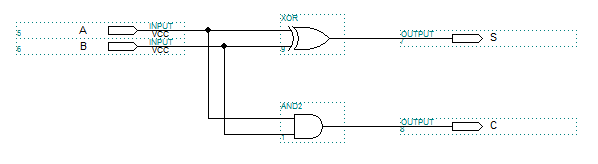
\includegraphics[scale=0.9]{half_adder.png}
%  \caption{Diagrama de um meio somador}
%\end{figure}


\FloatBarrier
\end{document}
